\documentclass[11pt]{article}
\addtolength{\oddsidemargin}{-1.cm}
\addtolength{\textwidth}{2cm}
\addtolength{\topmargin}{-2cm}
\addtolength{\textheight}{3.5cm}

\usepackage[pdftex]{graphicx}
\usepackage{hyperref}
\usepackage{float}
\usepackage{cite}
\hypersetup{
	colorlinks=true,
	linkcolor=black,
	filecolor=magenta,
	urlcolor=cyan,
}

% define the title
\author{Team CodeX}
\title{Functional Requirements Specification}

\begin{document}
	\setlength{\parskip}{6pt}
	
	% generates the title
	\begin{titlepage}
	
	\begin{center}
		% Upper part of the page       
		
\includegraphics[width=0.7\linewidth]{../Images/eVoting_Logo.png}\\[2cm]    
		\textsc{\LARGE Electronic Voting}\\[0.5cm]
		% Title
		\rule{\linewidth}{0.5mm} \\[1cm]
		{ \huge \bfseries User Manual}\\[0.5cm]
		\rule{\linewidth}{0.5mm} \\[1cm]
		
		% Author and supervisor
<<<<<<< HEAD
		
\includegraphics[width=0.5\linewidth]{../Images/TeamCodexLogo.jpg}\\[0.5cm]    	
=======
		
		
\includegraphics[width=0.5\textwidth]{../Images/TeamCodexLogo.jpg}\\[0.5cm]    	
>>>>>>> 9b25dd959830e00c0e449a84c7623c3e326c347b
		
		
		\begin{minipage}{0.4\textwidth}
			\begin{flushleft} \large
				Andreas {du Preez}
			\end{flushleft}
		\end{minipage}
		\begin{minipage}{0.4\textwidth}
			\begin{flushright} \large
				\emph{} \\
				12207871 
			\end{flushright}
		\end{minipage}
		
		
		\begin{minipage}{0.4\textwidth}
			\begin{flushleft} \large
				\emph{} \\
				Azhar {Mohungoo }
			\end{flushleft}
		\end{minipage}
		\begin{minipage}{0.4\textwidth}
			\begin{flushright} \large
				\emph{} \\
				12239799
			\end{flushright}
		\end{minipage}
		
		
		\begin{minipage}{0.4\textwidth}
			\begin{flushleft} \large
				\emph{} \\
				Gift {Sefako }
			\end{flushleft}
		\end{minipage}
		\begin{minipage}{0.4\textwidth}
			\begin{flushright} \large
				\emph{} \\
				12231097
			\end{flushright}
		\end{minipage}
		
		\textsc{\Large Stakeholders}\\[1cm]	
				
		\begin{minipage}{0.4\textwidth}
			\begin{flushleft} \large
				\emph{} \\
				Epi-Use Advance
			\end{flushleft}
		\end{minipage}
		\begin{minipage}{0.4\textwidth}
			\begin{flushright} \large
				\emph{} \\
				Roelof Nuade
			\end{flushright}
		\end{minipage}
		
	\end{center}
\end{titlepage}
	
	\tableofcontents
	\newpage
	
	\listoffigures
	\newpage
	
	\section{Introduction}
		This document aims to specify the functional and non-functional requirements as well as the architectural requirements for an electronic voting system specified by CodeX and the client EpiUse.

It will serve as a means of communication between the client and developers as well as providing an elaboration and a clear description of its implementation specifications.
	
	\section{Vision}
		What is intended for this project is to create a web and mobile platform, which can be used to cast votes in the provincial and national elections of South Africa. The following are benefits of the system:
	
	\begin{enumerate}
		\item The use of the Blockchain will allow for a transparent election process while still maintaining anonymity of the voters. 
		\item Votes that get lost or disgarded be it on purpose or not.
		\item Incorrect counting.
		\item Manual vote counting will no longer be required
		\item Remote casting of votes from a users preferred web browser or mobile smartphone. 
		\item Secure voting
		\item Prevent invalid votes from being cast through robust validation with each request.
	\end{enumerate}
	
	\section{Background}
		Elections are always a time where emotions are at a high and passion for a leader has never been greater. Sometimes this emotion and passion for a leader can lead to unlawful activities to get their chosen leader to to win the elections. By moving the system to an electronic environment it removes almost, if not all, these possibilities for unlawful activities to take place by using computers instead of humans. Although with the use of the Blockchain implementation, these activities can be suppressed.
	
Additionally to a secure and safe voting environment that allows ease of access from the voter's mobile or web browser, it will also make the voting process more efficient, with shorter queues to cast a vote and the progress of elections and the final result will be presented more rapidly, with periodic updates as the system analyses these votes. This system can be used in multiple scenarios not only in election. 

A more generic version of the electronic voting system can be implemented to allow users to partake in surveys, where instead of an election poll, users can create their own custom polls in which they can control participation. A further instance would be using such a system for national wide statistics, gathered by completing a poll of some kind, where anonymity is vital.
		\newpage
		
	\section{Functional Requirements}
	\begin{figure}[H]
		\centering
		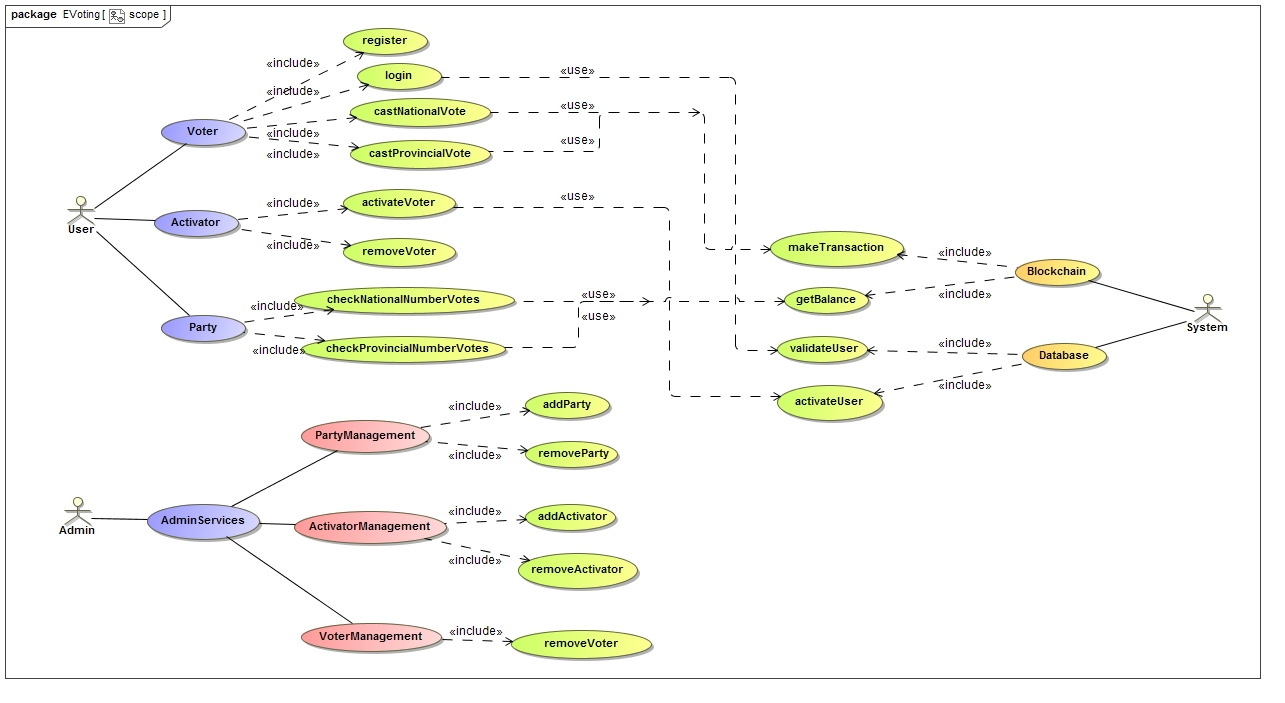
\includegraphics[width=\linewidth]{../Images/System/Scope.jpg}
		\caption{Scope Diagram}
	\end{figure}
	
	\newpage

	\subsection{Blockchain}
		\begin{enumerate}
	\item \textbf{Send Vote}
		\begin{enumerate}
			\item \textbf{Service Contract}
				\begin{figure}[H]
					\centering
					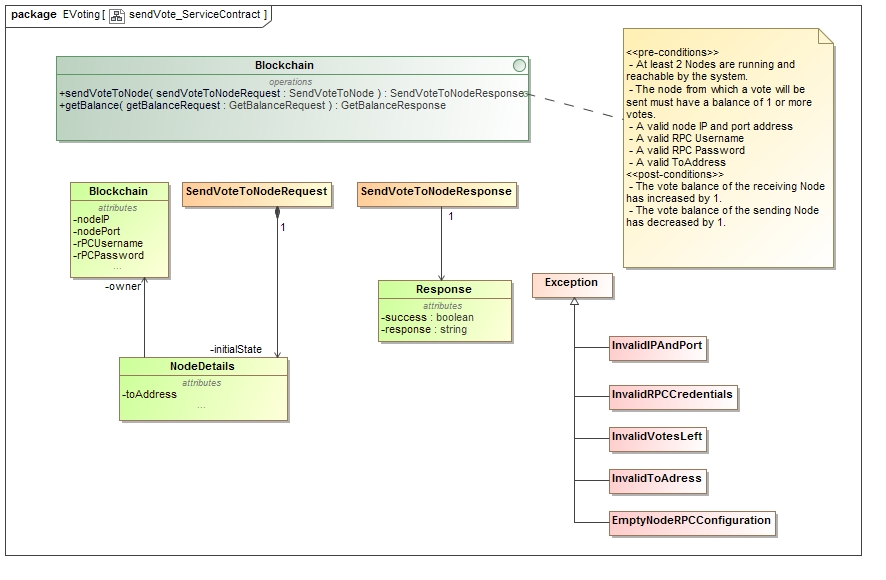
\includegraphics[width=0.75\linewidth]{../Images/Blockchain/ServiceContracts/sendVote_ServiceContract.jpg}
					\caption{Send Vote Service Contract}
				\end{figure}
				
				SendVote requires a ToAddress string which is the receiving node's address. The BlockchainModule is required to be instantiated with a NodeIP string, NodePort string, RPC username string and a RPC password string from where the vote will be sent.
				\newline				
				
				\begin{enumerate}
					\item Pre-conditions
					\begin{itemize}
						\item At least 2 Nodes are running and reachable by the system.
						\item The node from which a vote will be sent must have a balance of at least 1.
						\item A valid node IP and port address.
						\item A valid RPC Username.
						\item A valid RPC Password.
						\item A valid toAddress.
					\end{itemize}
					
					\item Exceptions
					\begin{itemize}
						\item If the configuration strings(node IP address, port address, RPC Username, RPC Password and toAddress) are empty, the EmptyNodeRPCConfiguration exception will be thrown.
						\item If the system cannot reach the node specified by the IP and port address, the InvalidIPAndPort exception will be thrown.
						\item If the specified RPC credentials are incorrect, the InvalidRPCCredentials exception will be thrown.
						\item If toAddress does not exist in the blockchain, the InvalidToAddress exception will be thrown.
						\item If the sending node does not have a balance of at least 1, the InvalidVotesLeft exception will be thrown.
					\end{itemize}
					
					\item Post-conditions
					\begin{itemize}
						\item The vote balance of the receiving node has increased by 1.
						\item The vote balance of the sending node has decreased by 1.
					\end{itemize}
				\end{enumerate}

			
			\item \textbf{Functional Requirements}
				\begin{figure}[H]
					\centering
					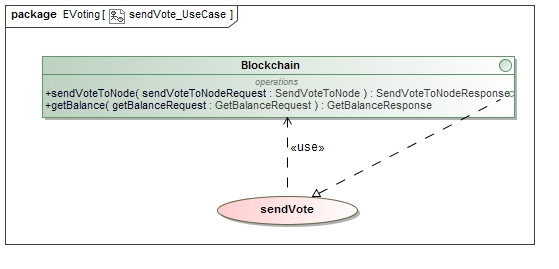
\includegraphics[width=0.75\linewidth]{../Images/Blockchain/UseCase/sendVote_UseCase.jpg}
					\caption{Send Vote Use Case}
				\end{figure}
				The sendVote process does not rely on any other use case, instead the sendVote process will be used by various other use cases.
				\newline
			\newpage
			\item \textbf{Process Design}
				\begin{figure}[H]
					\centering
					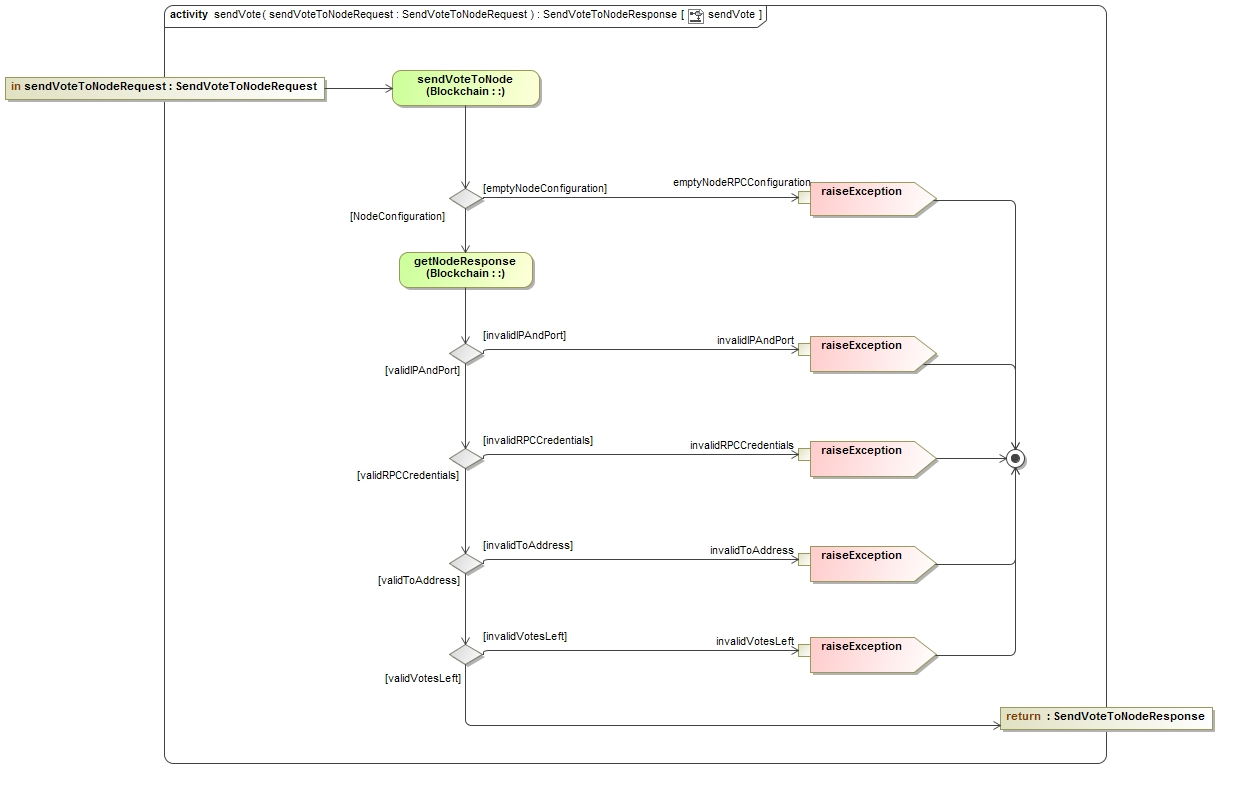
\includegraphics[width=0.75\linewidth]{../Images/Blockchain/Activity/sendVote.jpg}
					\caption{Send Vote Activity}
				\end{figure}
				Once the Send Vote process is called, it first checks if it has all the necesary configuration strings in order to send a vote. If any of these configuration strings are empty, an exception will be thrown. Sencondly the system will check if the node is reachable by sending it a 'ping' request and await a response. If the node does not respond, an exception will be thrown.
				The system will then try to make a transaction in the blockchain from the sending node to the receiving node. If the RPC credentials are incorrect, the InvalidRPCCredentials exception will be thrown. If the ToAddress does not exist in the blockchain, the InvalidToAddress exception will be thrown. If the sending node does not have atleast a balance of 1, the InvalidVotesLeft exception will be thrown. If no exceptions are thrown, and the node returns a string containing the transaction hash, it means the vote has been successfully sent.
				\newline
		\end{enumerate}
	\newpage
	\item \textbf{Get Balance}
		\begin{enumerate}
			\item \textbf{Service Contract}
			\begin{figure}[H]
				\centering
				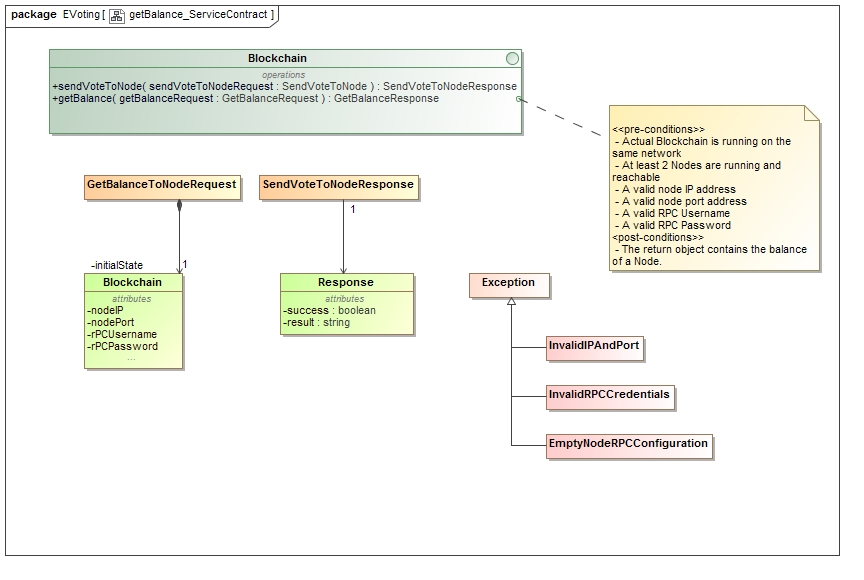
\includegraphics[width=0.75\linewidth]{../Images/Blockchain/ServiceContracts/getBalance_ServiceContract.jpg}
				\caption{Get Balance Service Contract}
			\end{figure}
			 
			In order for a political party to check how many votes they have, the system can return the balance of a specified node. The getBalance process returns the balance of the node specified by the configuration strings (nodeIP and nodePort).
			\newline
			
			\begin{enumerate}
				\item Pre-conditions
				\begin{itemize}
						\item At least 1 Node are running and reachable by the system.
						\item A valid node IP and port address.
						\item A valid RPC Username.
						\item A valid RPC Password.
				\end{itemize}
				
				\item Exceptions
				\begin{itemize}
						\item If the configuration strings(node IP address, port address, RPC Username, RPC Password) are empty, the EmptyNodeRPCConfiguration exception will be thrown.
						\item If the system cannot reach the node specified by the IP and port address, the InvalidIPAndPort exception will be thrown.
						\item If the specified RPC credentials are incorrect, the InvalidRPCCredentials exception will be thrown.
				\end{itemize}
				
				\item Post-conditions
				\begin{itemize}
					\item  The return object contains the balance of a Node in the 'reponse' field.
				\end{itemize}
			\end{enumerate}
			
			\newpage
			
			\item \textbf{Functional Requirements}
			\begin{figure}[H]
				\centering
				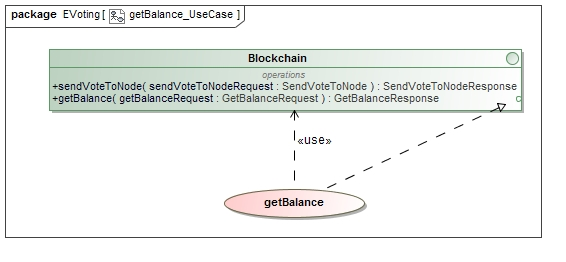
\includegraphics[width=0.75\linewidth]{../Images/Blockchain/UseCase/getBalance_UseCase.jpg}
				\caption{Get Balance Use Case}
			\end{figure}
			
			The getBalance process does not rely on any other use case, instead the Get Balance process will be used by various other use cases.
			\newline
			
			\item \textbf{Process Design}
			\begin{figure}[H]
				\centering
				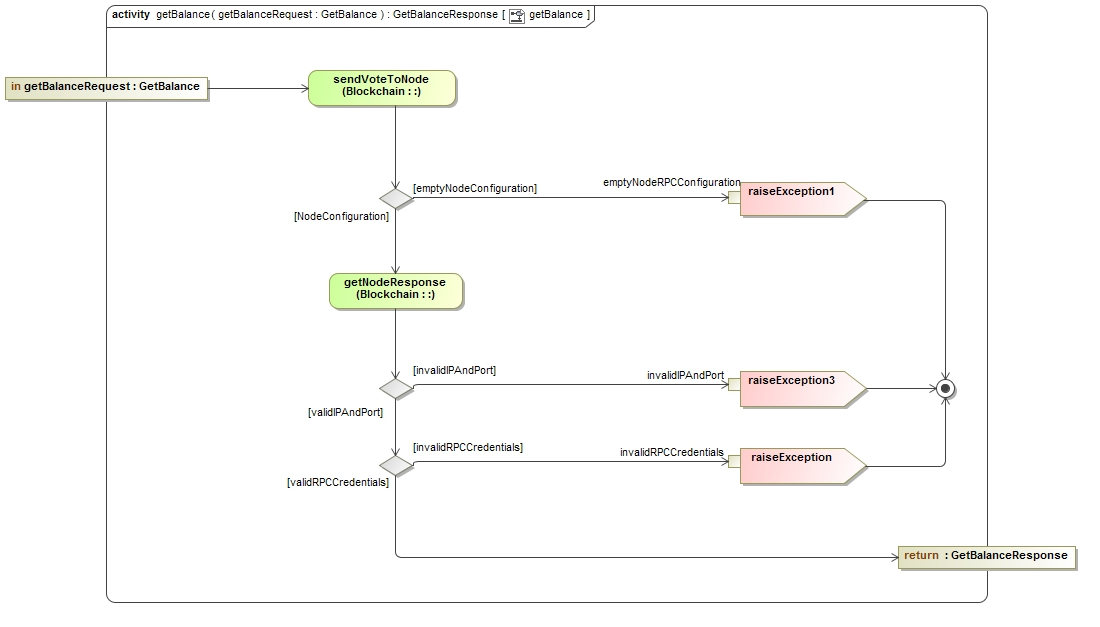
\includegraphics[width=0.75\linewidth]{../Images/Blockchain/Activity/getBalance.jpg}
				\caption{Get Balance Activity}
			\end{figure}
			
				When the getBalance process is called, it first checks if it has all the necesary configuration strings in order to connect to the node. If any of these configuration strings are empty, an exception will be thrown. Sencondly the system will check if the node is reachable by sending it a 'ping' request and await a response. If the node does not respond, an exception will be thrown.
				The system will then try to get the balance of the node. If the RPC credentials are incorrect, the InvalidRPCCredentials exception will be thrown. If no exceptions are thrown, the return object will contain the balance of that node.
			\newline
		\end{enumerate}
\end{enumerate}
		
	\subsection{Database}
		\begin{enumerate}
	\item \textbf{Validate User}
		\begin{enumerate}
			\item \textbf{Service Contract}
				\begin{figure}[H]
					\centering
					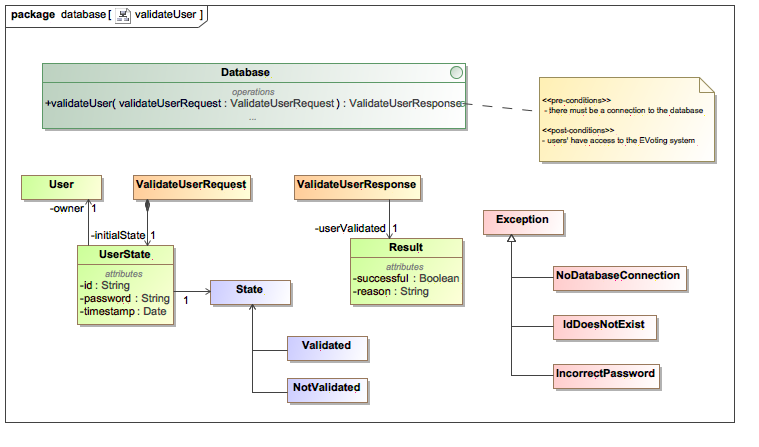
\includegraphics[width=0.75\linewidth]{../Images/Database/ServiceContracts/ValidateUser_ServiceContract.png}
					\caption{Validate User Service Contract}
				\end{figure}
								
				\begin{enumerate}
					\item Pre-conditions
					\begin{itemize}
						\item There must be a connection to the database
					\end{itemize}
					
					\item Exceptions
					\begin{itemize}
						\item If there is no connection to the database, the NoDatabaseConnection exception will be thrown
						\item If a user's ID is not valid, the IdDoesNotExist exception will be thrown
						\item If the user's password is entered incorrectly, the IncorrectPassword exception will be thrown
					\end{itemize}
					
					\item Post-conditions
					\begin{itemize}
						\item Users have access to the EVoting system
					\end{itemize}
				\end{enumerate}
			
			\newpage\textsl{}
			
			\item \textbf{Functional Requirements}
				\begin{figure}[H]
					\centering
					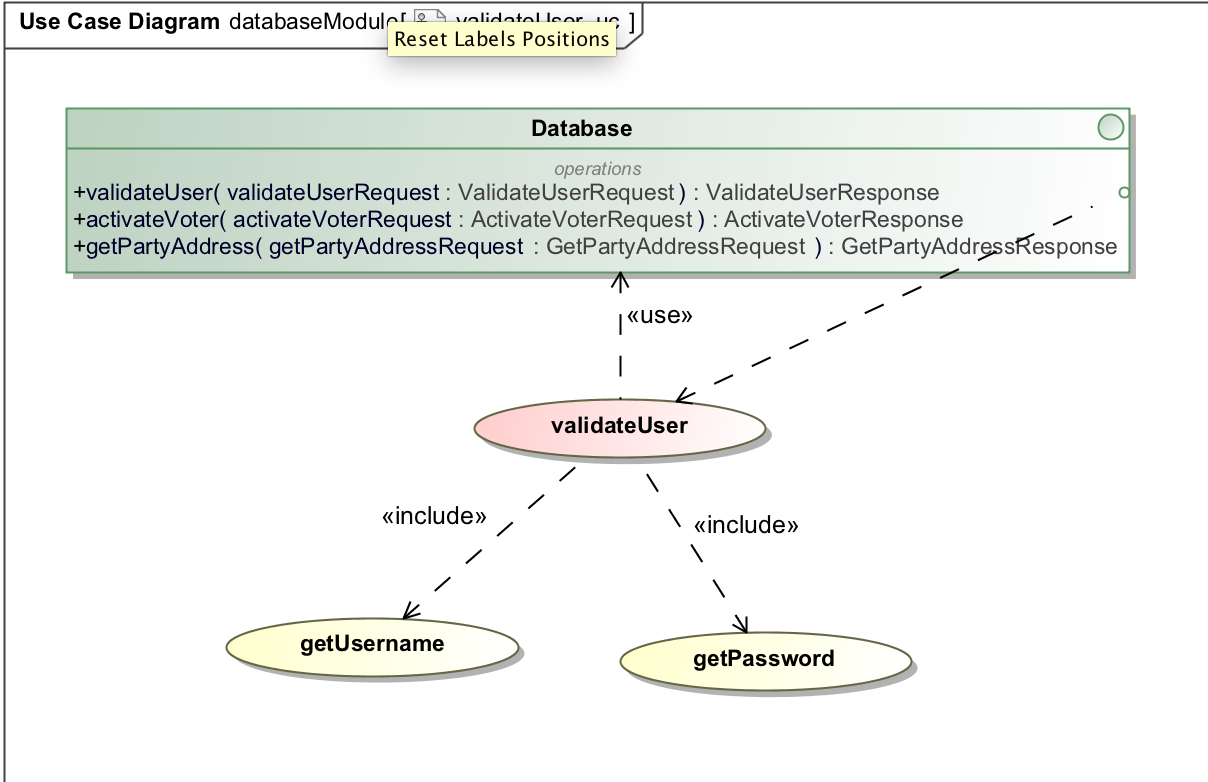
\includegraphics[width=0.75\linewidth]{../Images/Database/UseCases/ValidateUser_UseCase.png}
					\caption{Validate User Use Case}
				\end{figure}
				
			\item \textbf{Process Design}
				\begin{figure}[H]
					\centering
					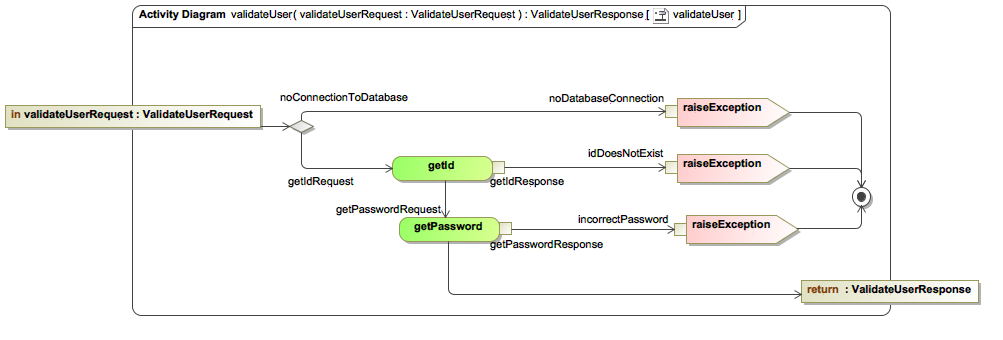
\includegraphics[width=0.75\linewidth]{../Images/Database/Activity/ValidateUser_Activity.png}
					\caption{Validate User Activity}
				\end{figure}
				
		\end{enumerate}
		
		\newpage
	
	\item \textbf{Activate User}
		\begin{enumerate}
			\item \textbf{Service Contract}
			\begin{figure}[H]
				\centering
				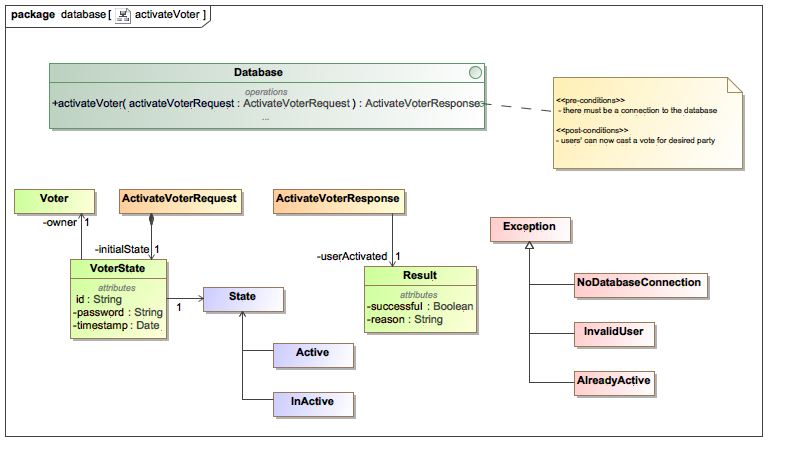
\includegraphics[width=0.75\linewidth]{../Images/Database/ServiceContracts/ActivateVoter_ServiceContract.png}
				\caption{Activate Voter Service Contract}
			\end{figure}
			
			\begin{enumerate}
				\item Pre-conditions
				\begin{itemize}
					\item There must be a connection to the database
				\end{itemize}
				
				\item Exceptions
				\begin{itemize}
						\item If there is no connection to the database, the NoDatabaseConnection exception will be thrown
						\item If a user could not be validated, the InvalidUser exception will be thrown
						\item If the user has already been activated, the AlreadyActive exception will be thrown
				\end{itemize}
				
				\item Post-conditions
				\begin{itemize}
					\item Users can now cast a vote for their desired party
				\end{itemize}
			\end{enumerate}
			
			\newpage
			
			\item \textbf{Functional Requirements}
			\begin{figure}[H]
				\centering
				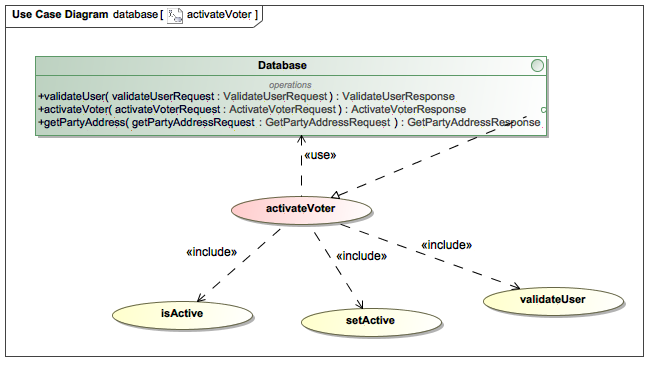
\includegraphics[width=0.75\linewidth]{../Images/Database/UseCases/ActivateVoter_UseCase.png}
				\caption{Activate Voter Use Case}
			\end{figure}
			
			\item \textbf{Process Design}
			\begin{figure}[H]
				\centering
				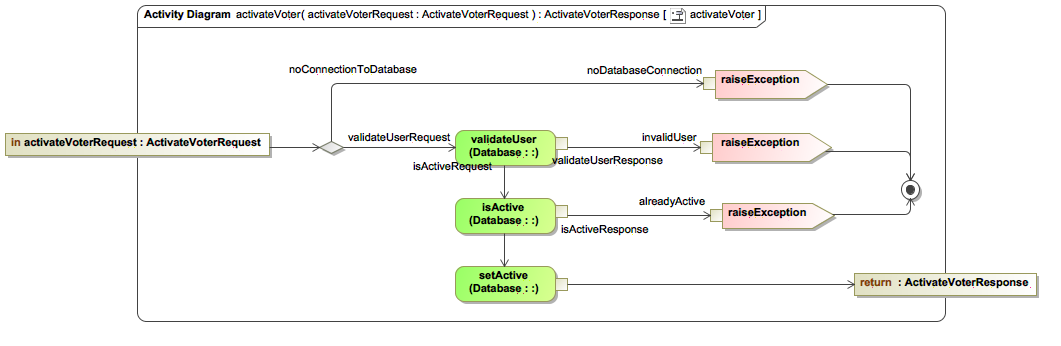
\includegraphics[width=0.75\linewidth]{../Images/Database/Activity/ActivateVoter_Activity.png}
				\caption{Activate Voter Activity}
			\end{figure}
			
		\end{enumerate}
\end{enumerate}
		
	\subsection{Admin}
		\begin{enumerate}
	\item \textbf{Deactivate Voter}
		\begin{enumerate}
			\item \textbf{Service Contract}
				\begin{figure}[H]
					\centering
					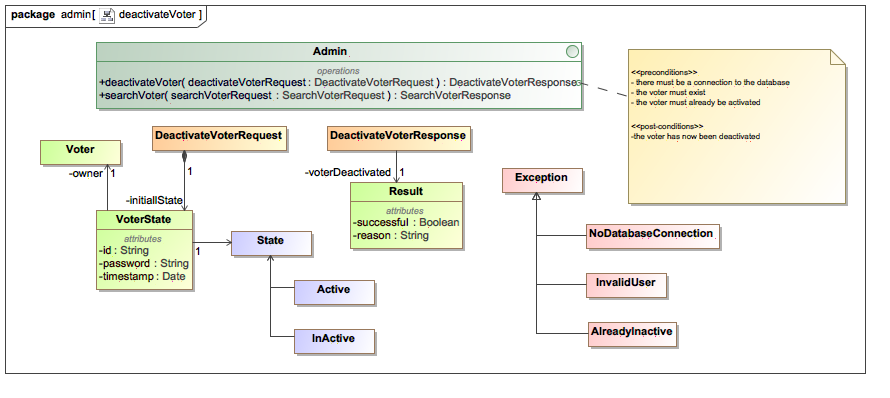
\includegraphics[width=0.75\linewidth]{../Images/Admin/ServiceContracts/deactivateVoter_ServiceContract.png}
					\caption{Deactivate Voter Service Contract}
				\end{figure}
				
				Deactivate Voter requires an ID number in the request which will be used to change the ActiveState state to inactive if all pre-conditions are met.
				\newline	
								
				\begin{enumerate}
					\item Pre-conditions
					\begin{itemize}
						\item There must be a connection to the database
						\item The voter must exist
						\item the voter must already be activated
					\end{itemize}
					
					\item Exceptions
					\begin{itemize}
						\item If there is no connection to the database, the NoDatabaseConnection exception will be thrown
						\item If a voter's ID is not valid, the IdDoesNotExist exception will be thrown
						\item If the voter is already active, the AlreadyActive exception will be thrown
					\end{itemize}
					
					\item Post-conditions
					\begin{itemize}
						\item The voter is now deactivated
					\end{itemize}
				\end{enumerate}
			
			\newpage\textsl{}
			
			\item \textbf{Functional Requirements}
				\begin{figure}[H]
					\centering
					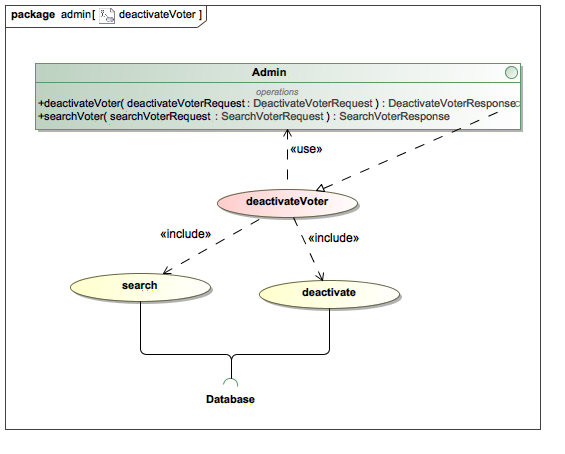
\includegraphics[width=0.75\linewidth]{../Images/Admin/UseCases/deactivateVoter_useCase.png}
					\caption{Deactivate Voter Use Case}
				\end{figure}
				
				The Deactivate Voter process will call the DeactivateVoter use case from the database module.
				\newline
				
			\item \textbf{Process Design}
				\begin{figure}[H]
					\centering
					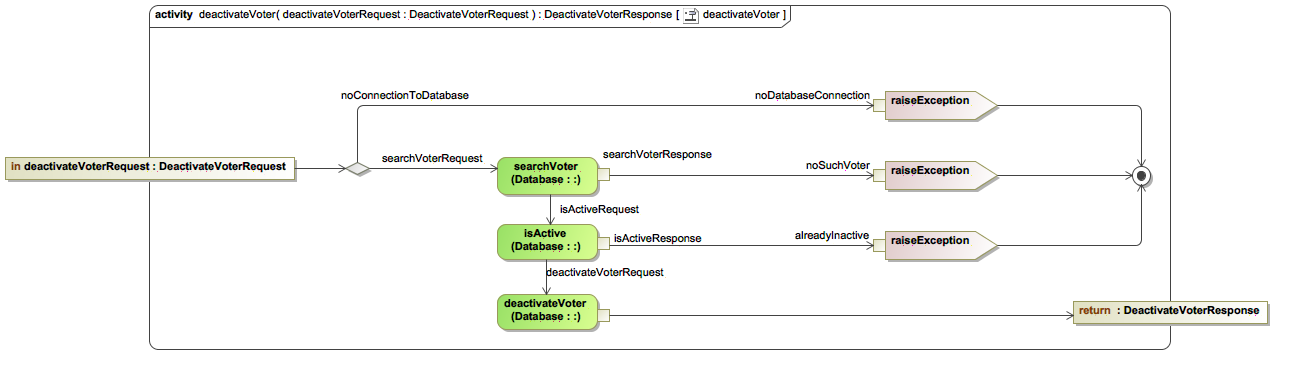
\includegraphics[width=0.75\linewidth]{../Images/Admin/ActivityDiagrams/deactivateVoter_ActivityDiagram.png}
					\caption{Deactivate Voter Activity}
				\end{figure}
				
				The Deactivate Voter process will first retrieve the ID number from the request and validate if is a valid ID number, after which it will get all the necessary Voter details from the database which corresponds to that ID number. It then checks in what state the voter is to see if it has already been deactivated. If all cases are valid, then the voter's ActiveState will change from Valid to Invalid.
				\newline
				
		\end{enumerate}
		
		\newpage
\end{enumerate}
		\newpage	
		
	\subsection{Voter}
		\begin{enumerate}
	\item \textbf{Register}
	
	Registering a Voter collects all the data required for a user to be valid and adds that information to the Voter database. Once the Voter has been added to the database they will have access to a minimum system. The minimum system only allows them to log in and view where they can go to get activated (to allow access to the entire system) to allow them to participate in the current election.
	
		\begin{enumerate}
			\item \textbf{Service Contract}
				\begin{figure}[H]
					\centering
					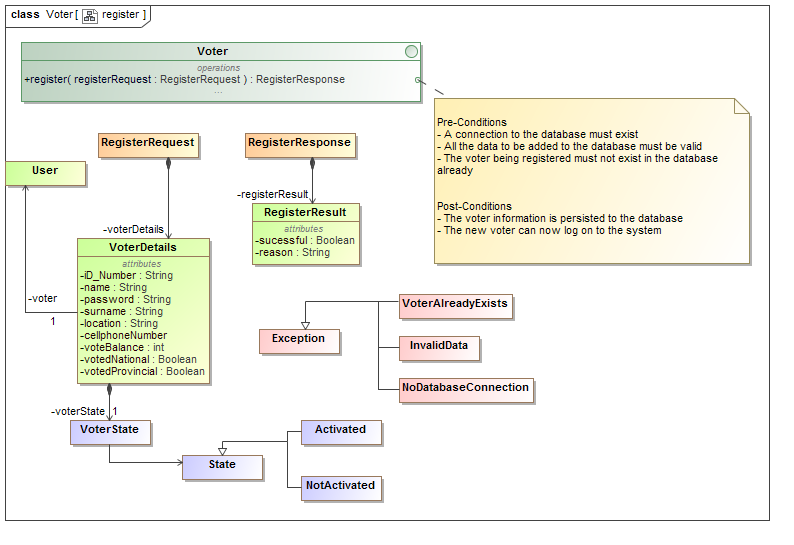
\includegraphics[width=0.75\linewidth]{../Images/Voter/ServiceContracts/register_serviceContract.png}
					\caption{Register Voter Service Contract}
				\end{figure}
				
			Register creates an initial state for a Voter and captures all the provided information in the database. Once information has been added to the database, the user can edit it themselves by accessing their account once they have logged in. Only valid data will be accepted. 
				\newline				
				
				\begin{enumerate}
					\item Pre-conditions
					\begin{itemize}
						\item There must be a connection to the database
						\item The information provided by the user must be valid.
						\item The user must not exist in the current database. 
					\end{itemize}
					
					\item Exceptions
					\begin{itemize}
						\item If there is no connection to the database, the NoDatabaseConnection exception will be thrown.
						\item If the data is invalid then the service is refused and the InvalidData exception is thrown.
						\item If the user already exists in the database then the service is refused and the UserAlreadyExists exception is thrown.
					\end{itemize}
					
					\item Post-conditions
					\begin{itemize}
						\item The new Voter can log in and access the Electronic Voting system. 
						\item The Voter’s information is persisted to the database.
					\end{itemize}
				\end{enumerate}
			
			\item \textbf{Functional Requirements}
				\begin{figure}[H]
					\centering
					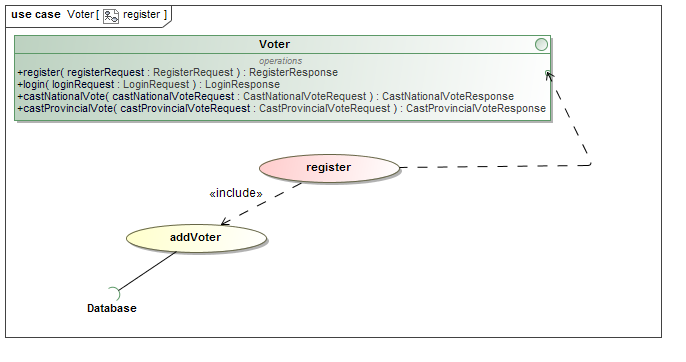
\includegraphics[width=0.75\linewidth]{../Images/Voter/UseCases/register_useCase.png}
					\caption{Register Voter Use-Case}
				\end{figure}
				
				\begin{enumerate}
					\item The registerRequest object encapsulates all the necessary information required to add a new Voter to the system. 
					\item All the information collected by the register function is persisted to the database through the Database module's addVoter function. 
				\end{enumerate}
				
			
			
			
			\item \textbf{Process Design}
				\begin{figure}[H]
					\centering
					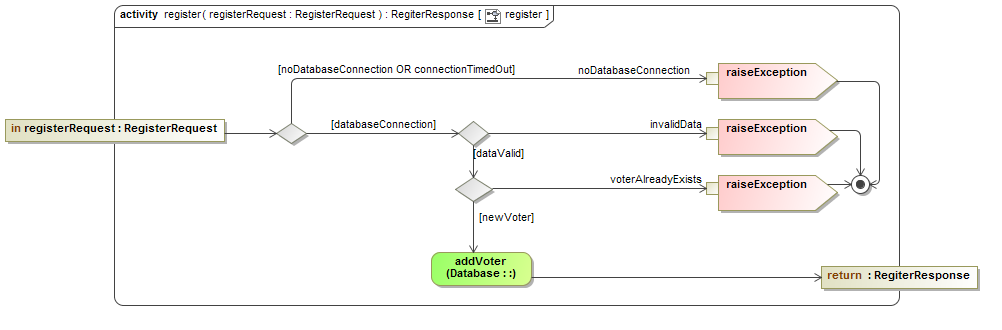
\includegraphics[width=0.75\linewidth]{../Images/Voter/ActivityDiagrams/register_activity.png}
					\caption{Register Voter Activity}
				\end{figure}
				
				\begin{enumerate}
					\item The Register function first checks to see if there is a connection to the database, if there is not or the connection times out, the NoDatabaseConnection exception is thrown. 
					\item If there is a database connection, it checks whether the Voter's data is valid(according to the data types specified in the database). 
					\item If the data is not valid, the InvalidData exception is thrown. 
					\item Then the function checks whether the Voter's information already exists in the database and throws the VoterAlreadyExists exception if the Voter already exists.
					\item Otherwise no exception is thrown and the Voter's information is persisted to the database using the Database module's addVoter function. 
					
				\end{enumerate}
				
				
\end{enumerate}
	
	\item \textbf{Login}
	
	Login functionality gives the user access to system and allows them to view their account information, and only once they have been activated, are they allowed to cast votes and view other relevant information. 
	
		\begin{enumerate}
			\item \textbf{Service Contract}
			\begin{figure}[H]
				\centering
				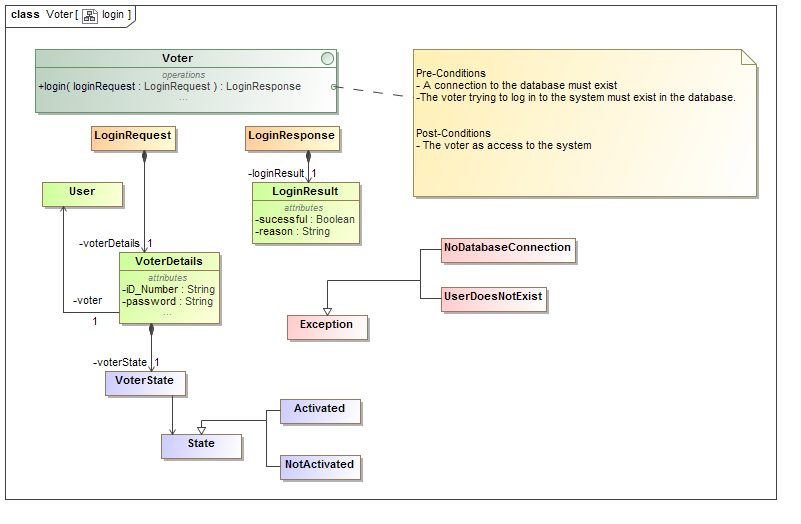
\includegraphics[width=0.75\linewidth]{../Images/Voter/ServiceContracts/login_serviceContract.png}
				\caption{Login Service Contract}
			\end{figure}
			
			Login validates a user and gives them rights to interact with the core system. 
			\newline
			
			\begin{enumerate}
				\item Pre-conditions
				\begin{itemize}
					\item There must be a connection to the database
					\item The user must have already registered. 
				\end{itemize}
				
				\item Exceptions
				\begin{itemize}
						\item If there is no connection to the database, the NoDatabaseConnection exception will be thrown
						\item If the user has not registered then the UserDoesNotExist exception is thrown and the service is denied. 
				\end{itemize}
				
				\item Post-conditions
				\begin{itemize}
					\item The Voter has access to the Electronic Voting system.
				\end{itemize}
			\end{enumerate}
			
			\newpage
			
			\item \textbf{Functional Requirements}
			\begin{figure}[H]
				\centering
				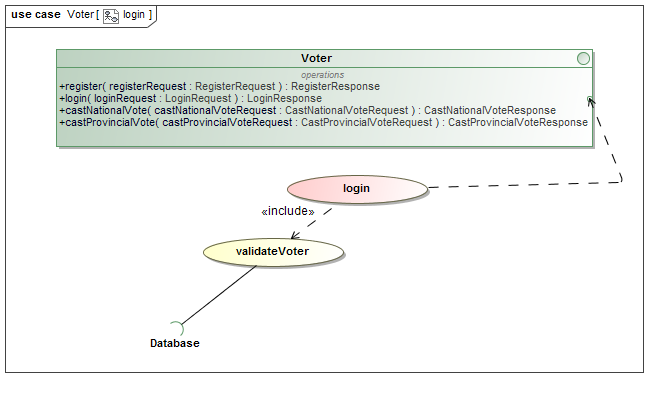
\includegraphics[width=0.75\linewidth]{../Images/Voter/UseCases/login_useCase.png}
				\caption{Login Voter Use-Case}
			\end{figure}
			
			\begin{enumerate}
				\item The login use-case collects Voter information which will be used to validate a Voter. 
				\item A Voter is invalid if their credentials do not checkout. 
				\item The Voter module's login passes information to the Database modules validateVoter function to check whether the Voter attempting to log in is valid or not.  
			\end{enumerate}
			
			\item \textbf{Process Design}
			\begin{figure}[H]
				\centering
				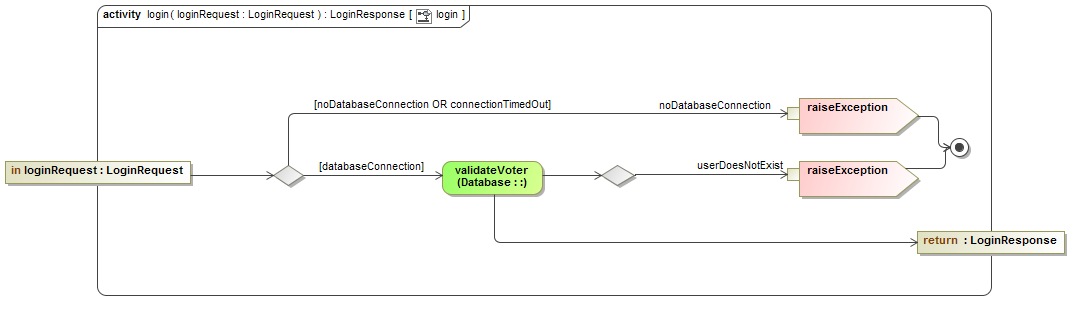
\includegraphics[width=0.75\linewidth]{../Images/Voter/ActivityDiagrams/login_activity.png}
				\caption{Login Voter Activity}
			\end{figure}
			
			
			\begin{enumerate}
				\item The Login function first checks to see if there is a connection to the database, if there is not or the connection times out, the NoDatabaseConnection exception is thrown.
				\item Then it calls the Database module's validateUser function which will return an object that contains a boolean value of whether the voter is valid (and can thus access the system) as well as a reason or false (thus the Voter is denied access) as well as reason as to why the service has been denied. 
				\item The UserDoesNotExist exception is thrown if validateUser returns false. 
			\end{enumerate}			
		\end{enumerate}

\newpage

	\item \textbf{Cast National Vote}
	
	Casting a vote requires voter to be logged in.
	
	\begin{enumerate}
		\item \textbf{Service Contract}
		\begin{figure}[H]
			\centering
			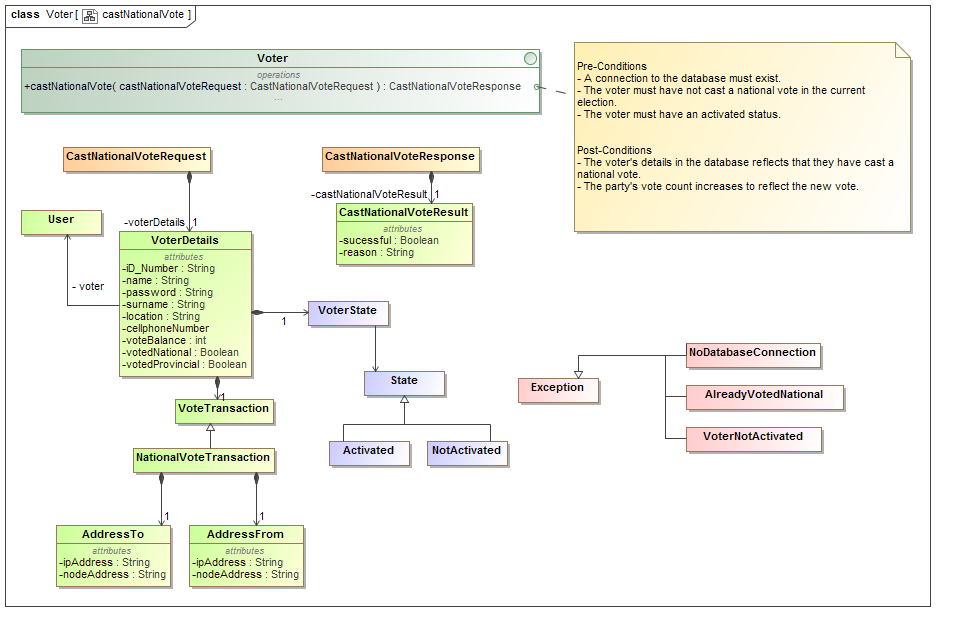
\includegraphics[width=0.75\linewidth]{../Images/Voter/ServiceContracts/castNationalVote_serviceContract.png}
			\caption{Cast National Vote Service Contract}
		\end{figure}
		
		Once the Voter is logged in we can retrieve their account information to view their location and their current vote balance(calculated by whether they have voted national, provincial or neither). \newline
	 The voting node’s address for the current voter(based on the user’s location) as well as the party node’s address are retrieved, this information will be sent to the Blockchain Module to concretely cast the voters vote as Blockchain transaction.
		\newline				
		
		\begin{enumerate}
			\item Pre-conditions
			\begin{itemize}
				\item There must be a connection to the database
				\item The Voter must not have already cast a National vote in the current election. 
				\item The Voter must have an Activated status.  
			\end{itemize}
			
			\item Exceptions
			\begin{itemize}
				\item If there is no connection to the database, the NoDatabaseConnection exception will be thrown.
				\item If the Voter has already cast a National vote, the AlreadyVotedNational exception is thrown and the service is denied.
				\item If the Voter has not been activated by an Activator, the VoterNotActivated exception is thrown and they are disallowed from casting a vote. 
			\end{itemize}
			
			\newpage
			
			\item Post-conditions
			\begin{itemize}
				\item Voter details in the database reflect that they have cast a National Vote. 
				\item The Party which the Voter has voted for shows an increment by one in their node balance. 
			\end{itemize}
		\end{enumerate}
		
		\item \textbf{Functional Requirements}
		\begin{figure}[H]
			\centering
			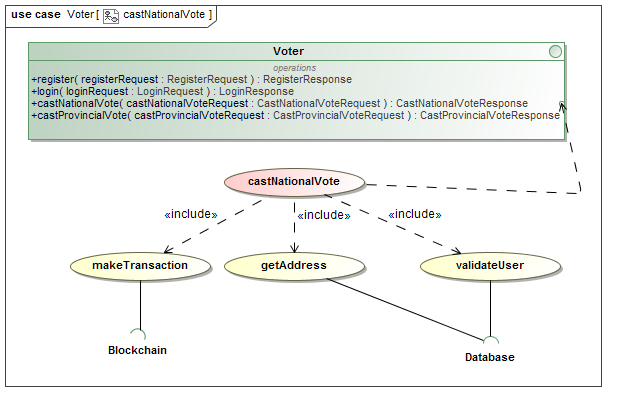
\includegraphics[width=0.75\linewidth]{../Images/Voter/UseCases/castNationalVote_useCase.png}
			\caption{Cast National Vote Use Case}
		\end{figure}
		
		\begin{enumerate}
			\item The Cast National Vote use case starts uses the database to retrieve the addresses of the Party which is being voted for as well as the Voting region node's addresses.   
			\item Once it has all the addresses, it uses the Blockchain's makeTransaction functionality to cast the vote into the Blockchain. (Sending one coin from the Voting Region Node to the coin accepting Party Node of the Voter's choice.) 
		\end{enumerate}
		
		\item \textbf{Process Design}
		\begin{figure}[H]
			\centering
			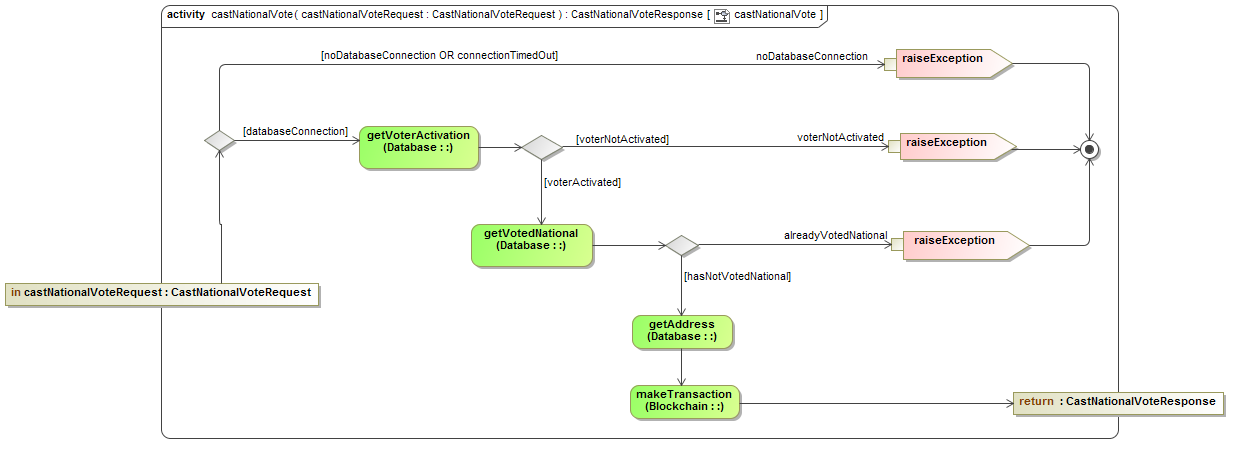
\includegraphics[width=0.75\linewidth]{../Images/Voter/ActivityDiagrams/castNationalVote_activity.png}
			\caption{Cast National Vote Activity}
		\end{figure}
		
		\begin{enumerate}
			\item The function first checks to see if there is a connection to the database, if there is not or the connection times out, the NoDatabaseConnection exception is thrown. 
			\item If a connection exists, it proceeds to check whether the Voter has been activated or not. 
			\item If the Voter has not been activated, the VoterNotActivated exception is thrown. 
			\item Then the function checks whether the Voter has already cast a National vote. If they have the AlreadyVotedNational exception is thrown.
			\item If none of the exceptions are thrown, the function then queries the database to find all of the necessary addresses then it calls the Blockchain's makeTransaction function to cast the actual vote.  
			
		\end{enumerate}
	\end{enumerate}

	\item \textbf{Cast Provincial Vote}
	
	Casting a vote requires voter to be logged in.
	
	\begin{enumerate}
		\item \textbf{Service Contract}
		\begin{figure}[H]
			\centering
			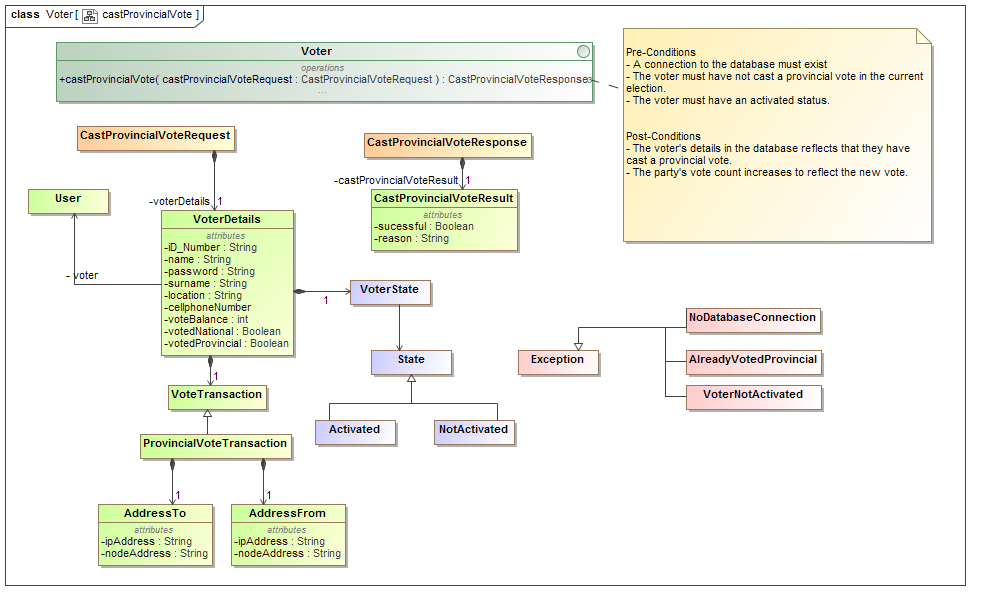
\includegraphics[width=0.75\linewidth]{../Images/Voter/ServiceContracts/castProvincialVote_serviceContract.png}
			\caption{Cast Provincial Vote Service Contract}
		\end{figure}
		
		Once the Voter is logged in we can retrieve their account information to view their location and their current vote balance(calculated by whether they have voted national, provincial or neither). \newline
		The voting node’s address for the current voter(based on the user’s location) as well as the party node’s address are retrieved, this information will be sent to the Blockchain Module to concretely cast the voters vote as Blockchain transaction.
		\newline				
		
		\begin{enumerate}
			\item Pre-conditions
			\begin{itemize}
				\item There must be a connection to the database
				\item The Voter must not have already cast a Provincial vote in the current election. 
				\item The Voter must have an Activated status.  
			\end{itemize}
			
			\item Exceptions
			\begin{itemize}
				\item If there is no connection to the database, the NoDatabaseConnection exception will be thrown.
				\item If the Voter has already cast a National vote, the AlreadyVotedProvincial exception is thrown and the service is denied.
				\item If the Voter has not been activated by an Activator, the VoterNotActivated exception is thrown and they are disallowed from casting a vote. 
			\end{itemize}
			
			\item Post-conditions
			\begin{itemize}
				\item Voter details in the database reflect that they have cast a Provincial Vote. 
				\item The Party which the Voter has voted for shows an increment by one in their node balance. 
			\end{itemize}
		\end{enumerate}
		
		\item \textbf{Functional Requirements}
		\begin{figure}[H]
			\centering
			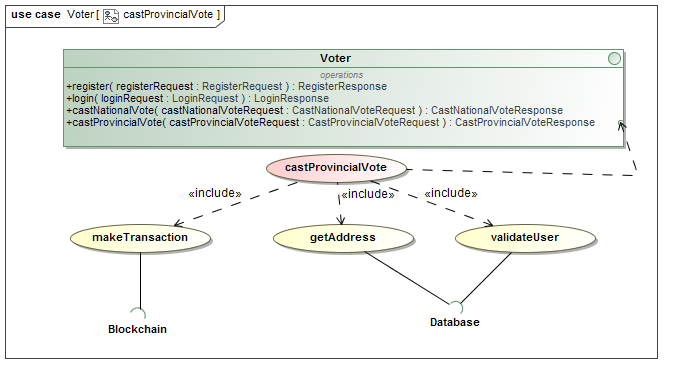
\includegraphics[width=0.75\linewidth]{../Images/Voter/UseCases/castProvincialVote_useCase.png}
			\caption{Cast Provincial Vote Use Case}
		\end{figure}
		
		\begin{enumerate}
			\item The Cast Provincial Vote use case starts uses the database to retrieve the addresses of the Party which is being voted for as well as the Voting region node's addresses.   
			\item Once it has all the addresses, it uses the Blockchain's makeTransaction functionality to cast the vote into the Blockchain. (Sending one coin from the Voting Region Node to the coin accepting Party Node of the Voter's choice.) 
		\end{enumerate}
		
		\newpage
		
		\item \textbf{Process Design}
		\begin{figure}[H]
			\centering
			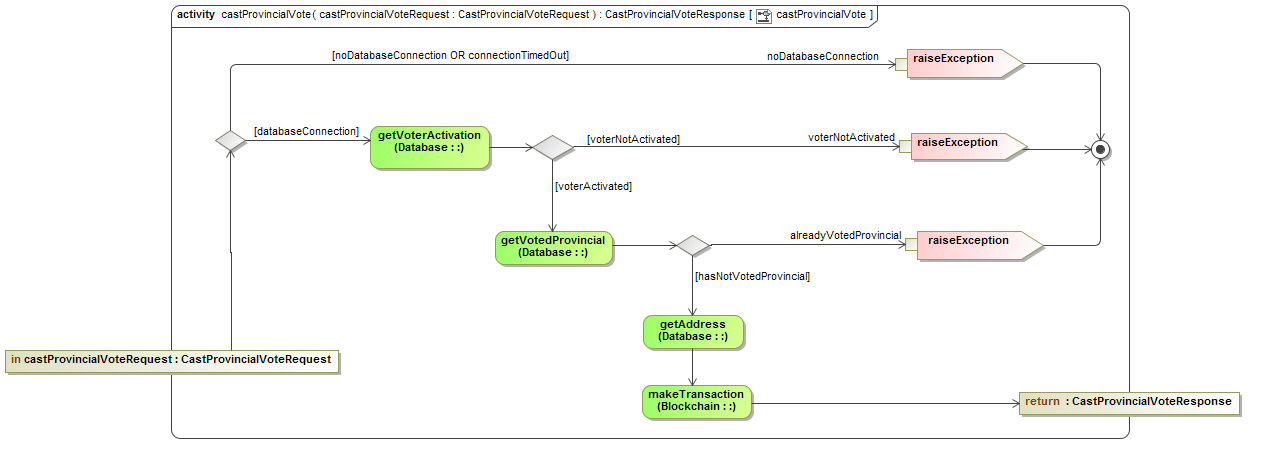
\includegraphics[width=0.75\linewidth]{../Images/Voter/ActivityDiagrams/castProvincialVote_activity.png}
			\caption{Cast Provincial Vote Activity}
		\end{figure}
		
		\begin{enumerate}
			\item The function first checks to see if there is a connection to the database, if there is not or the connection times out, the NoDatabaseConnection exception is thrown. 
			\item If a connection exists, it proceeds to check whether the Voter has been activated or not. 
			\item If the Voter has not been activated, the VoterNotActivated exception is thrown. 
			\item Then the function checks whether the Voter has already cast a Provincial vote. If they have the AlreadyVotedProvincial exception is thrown.
			\item If none of the exceptions are thrown, the function then queries the database to find all of the necessary addresses then it calls the Blockchain's makeTransaction function to cast the actual vote.  
			
		\end{enumerate}
	\end{enumerate}
\end{enumerate}










		\newpage
		
	\subsection{Activator}
		\begin{enumerate}
	\item \textbf{Activate Voter}
		\begin{enumerate}
			\item \textbf{Service Contract}
				\begin{figure}[H]
					\centering
					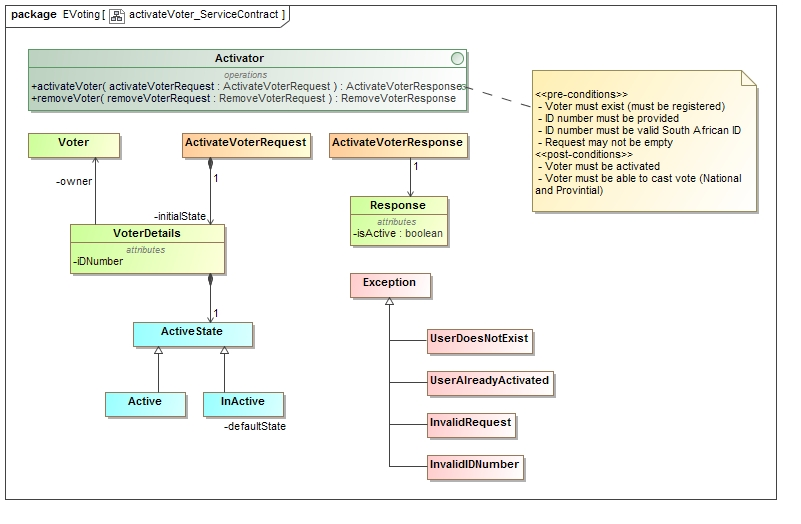
\includegraphics[width=0.75\linewidth]{../Images/Activator/ServiceContract/activateVoter_ServiceContract.jpg}
					\caption{Activate Voter Service Contract}
				\end{figure}
				
				Activate Voter requires an ID number in the request which will be used to change the ActiveState state to active if all pre-conditions are met.
				\newline				
				
				\begin{enumerate}
					\item Pre-conditions
					\begin{itemize}
						\item An ID number must be present in the request.
						\item The ID number must be a valid South African ID number.
						\item Voter must exist (must be a registered voter).
						\item The voter must not already be registered.
					\end{itemize}
					
					\item Exceptions
					\begin{itemize}
						\item If the ID number is not a valid South African ID, the invalidIDNumber exception will be thrown.
						\item If the user does not exist in the database, the userDoesNotExist exception will be thrown.
						\item If the user is already activated, the userAlreadyActivated exception will be thrown.
					\end{itemize}
					
					\item Post-conditions
					\begin{itemize}
						\item The Voter's ActivateState must be Active.
					\end{itemize}
				\end{enumerate}
			
			\newpage
			
			\item \textbf{Functional Requirements}
				\begin{figure}[H]
					\centering
					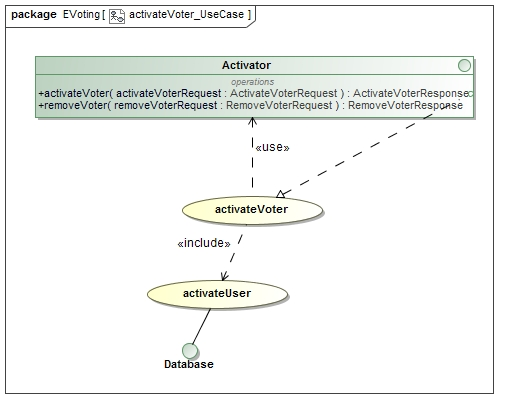
\includegraphics[width=0.75\linewidth]{../Images/Activator/UseCase/activateVoter_UseCase.jpg}
					\caption{Activate User Use Case}
				\end{figure}
				
				The Activate Voter process will call the ActivateUser use case from the database module.
				\newline
			
			\item \textbf{Process Design}
				\begin{figure}[H]
					\centering
					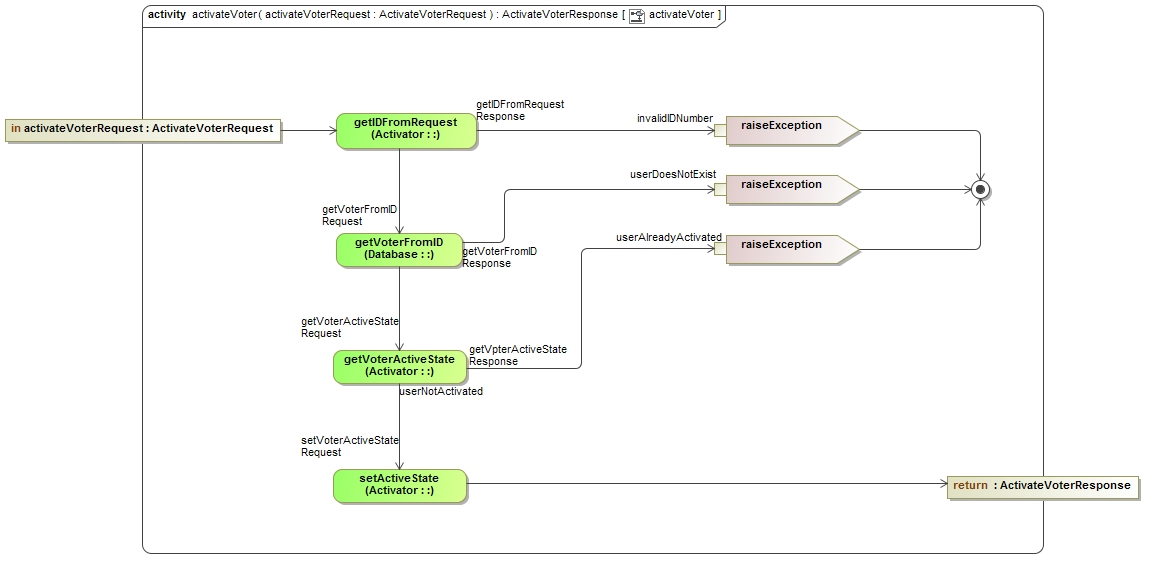
\includegraphics[width=0.75\linewidth]{../Images/Activator/Activity/activateVoter.jpg}
					\caption{Activate User Activity}
				\end{figure}
				
				The Activate Voter process will first retrieve the ID number from the request and validate if is a valid ID number, after which it will get all the necessary Voter details from the database wich corresponds to that ID number. It then checks in what state the voter is to see if it has already been activated. If all cases are valid, then the voter's ActiveState will change from Invalid to Valid.
				\newline
		\end{enumerate}
	
	\item \textbf{Remove Voter}
		\begin{enumerate}
			\item \textbf{Service Contract}
			\begin{figure}[H]
				\centering
				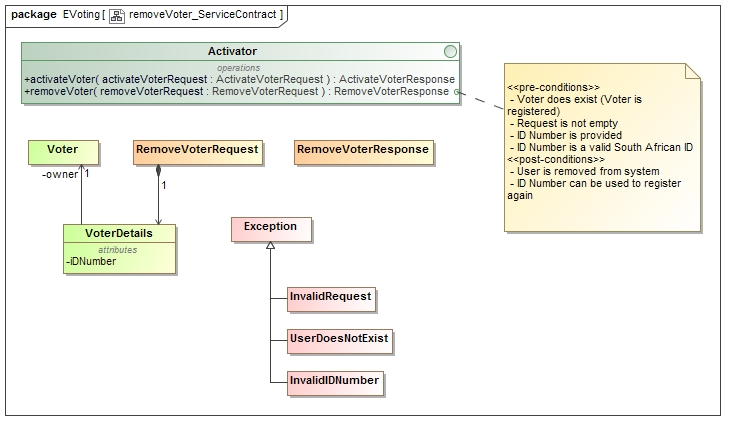
\includegraphics[width=0.75\linewidth]{../Images/Activator/ServiceContract/removeVoter_ServiceContract.jpg}
				\caption{Remove Voter Service Contract}
			\end{figure}
			
			There are cases where the Activator will need to be able to remove a user. In the removeActivatorRequest, an ID number must be provided so that the voter associated with that ID number be removed from the system.
			\newline
			
			\begin{enumerate}
				\item Pre-conditions
				\begin{itemize}
					\item An ID number must be provided.
					\item The ID number must be a valid South African ID.
					\item The user must exist in the system.
				\end{itemize}
				
				\item Exceptions
				\begin{itemize}
						\item If the ID number in the request is not a valid ID number, the InvalidIDNumber exception will be thrown.
						\item If the user does not exist in the database, the userDoesNotExist exception will be thrown.
				\end{itemize}
				
				\item Post-conditions
				\begin{itemize}
					\item The user is removed from the system.
				\end{itemize}
			\end{enumerate}
			
			\newpage
			
			\item \textbf{Functional Requirements}
			\begin{figure}[H]
				\centering
				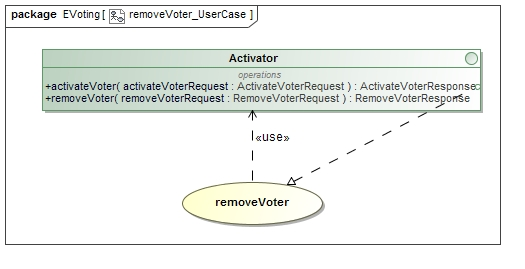
\includegraphics[width=0.75\linewidth]{../Images/Activator/UseCase/removeVoter_UserCase.jpg}
				\caption{Remove Voter Use Case}
			\end{figure}
			
			The removeVoter will call a method of the database to remove the voter with that ID number. The database module is not fully documented as of yet.
			\newline
			
			\item \textbf{Process Design}
			\begin{figure}[H]
				\centering
				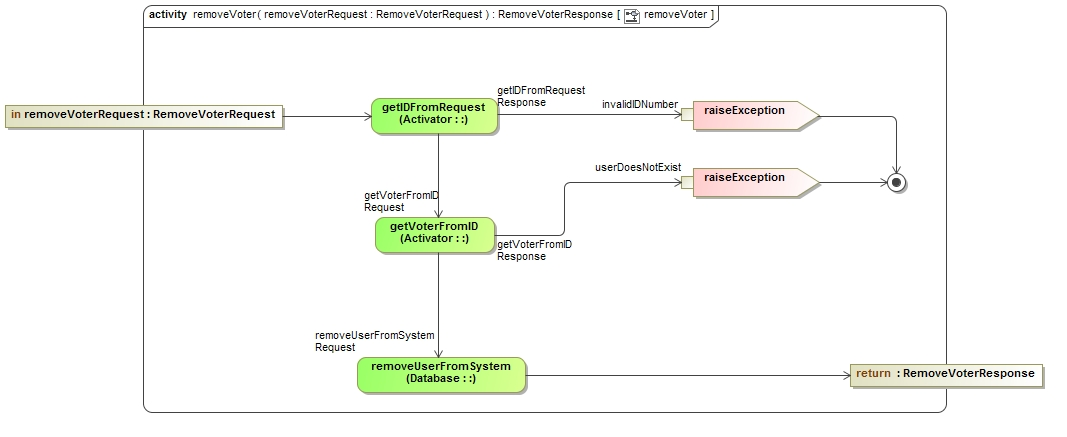
\includegraphics[width=0.75\linewidth]{../Images/Activator/Activity/removeVoter.jpg}
				\caption{Remove Voter Activity}
			\end{figure}
			
				The Remove Voter process will first retrieve the ID number from the request and validate if is a valid ID number. If a user associated with that ID number is found, the process will call a function from the database module to remove the user from the system.
			\newline
		\end{enumerate}
\end{enumerate}
		\newpage
		
	\subsection{Party}
		\begin{enumerate}
	\item \textbf{Check National Number Votes}
		\begin{enumerate}
			\item \textbf{Service Contract}
				\begin{figure}[H]
					\centering
					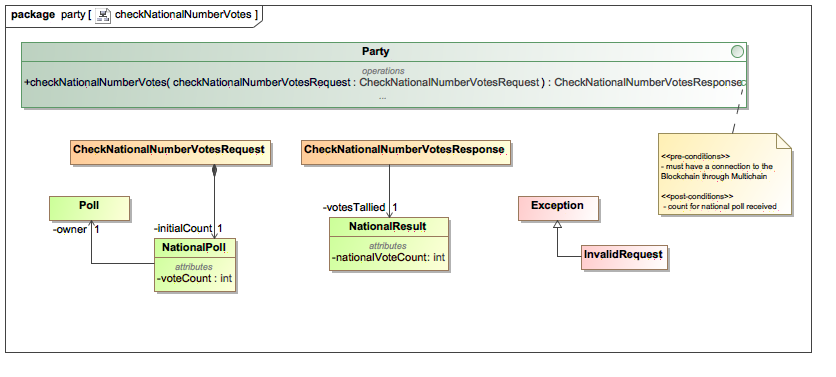
\includegraphics[width=0.75\linewidth]{../Images/Party/ServiceContracts/CheckNationalNumberVotes_ServiceContract.png}
					\caption{Check National Number Votes Service Contract}
				\end{figure}
				
				The system queries the number of national votes a Party has acquired in total.
				\newline				
				\begin{enumerate}
					\item Pre-conditions
					\begin{itemize}
						\item There must be a connection to the Blockchain through the Multichain
					\end{itemize}
					
					\item Exceptions
					\begin{itemize}
						\item If there is no connection to the Blockchain, the InvalidRequest exception will be thrown
					\end{itemize}
					
					\item Post-conditions
					\begin{itemize}
						\item The count for the National Poll is received
					\end{itemize}
				\end{enumerate}
			
			\item \textbf{Functional Requirements}
				\begin{figure}[H]
					\centering
					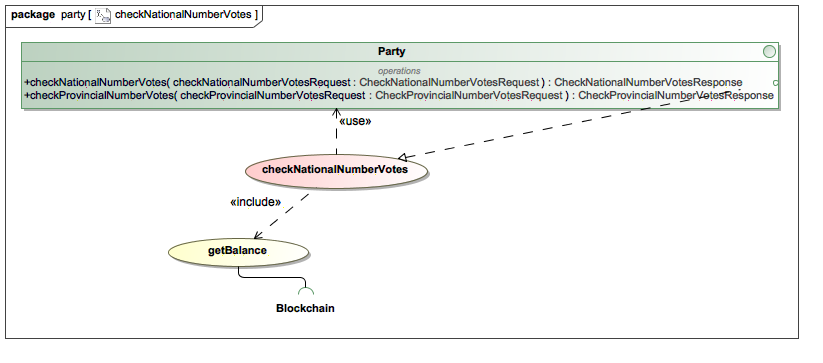
\includegraphics[width=0.75\linewidth]{../Images/Party/UseCases/CheckNationalNumberVotes_UseCase.png}
					\caption{Check National Number Votes Use Case}
				\end{figure}
				
				\newpage
				
			\item \textbf{Process Design}
				\begin{figure}[H]
					\centering
					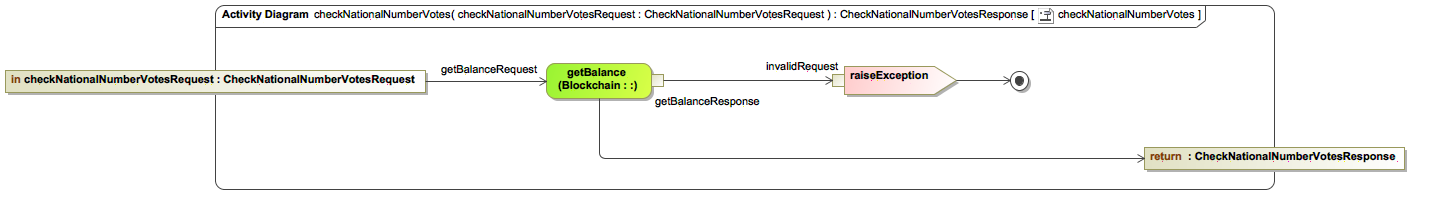
\includegraphics[width=0.75\linewidth]{../Images/Party/ActivityDiagrams/CheckNationalNumberVotes_Activity.png}
					\caption{Check National Number Votes Activity}
				\end{figure}
				
		\end{enumerate}
	
	\item \textbf{Check Provincial Number Votes}
		\begin{enumerate}
			\item \textbf{Service Contract}
			\begin{figure}[H]
				\centering
				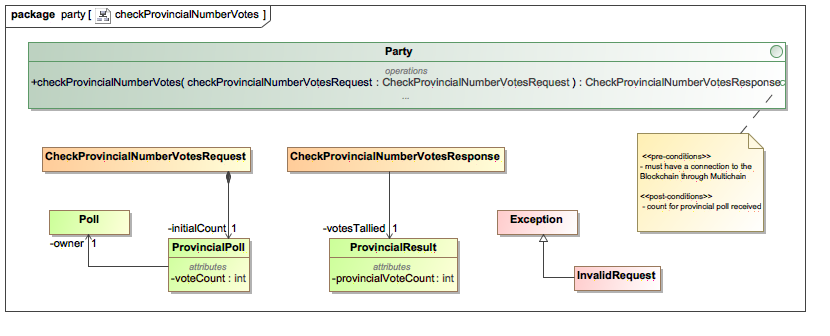
\includegraphics[width=0.75\linewidth]{../Images/Party/ServiceContracts/CheckProvincialNumberVotes_ServiceContract.png}
				\caption{Check National Number Votes Service Contract}
			\end{figure}
			
			The system queries the number of provincial votes a Party has acquired in total.
			\newline
			
			\begin{enumerate}
				\item Pre-conditions
				\begin{itemize}
					\item There must be a connection to the Blockchain through the Multichain
				\end{itemize}
				
				\item Exceptions
				\begin{itemize}
						\item If there is no connection to the Blockchain, the InvalidRequest exception will be thrown
				\end{itemize}
				
				\item Post-conditions
				\begin{itemize}
					\item The count for the Provincial Poll is received
				\end{itemize}
			\end{enumerate}
			\newpage
			\item \textbf{Functional Requirements}
			\begin{figure}[H]
				\centering
				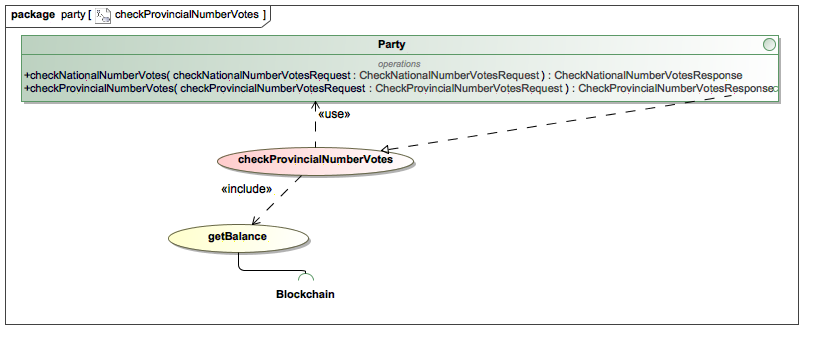
\includegraphics[width=0.75\linewidth]{../Images/Party/UseCases/CheckProvincialNumberVotes_UseCase.png}
				\caption{Check National Number Votes Use Case}
			\end{figure}
						
			\item \textbf{Process Design}
			\begin{figure}[H]
				\centering
				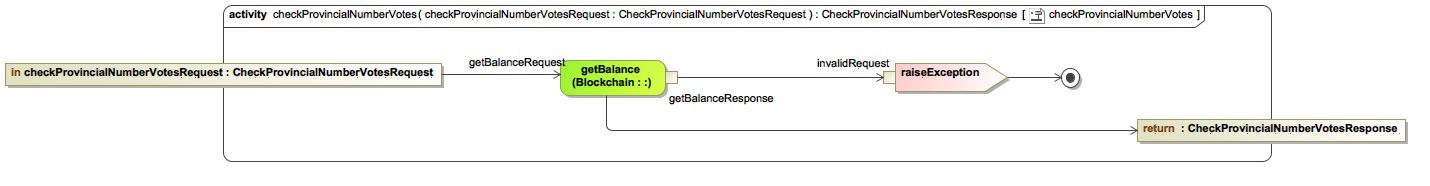
\includegraphics[width=0.75\linewidth]{../Images/Party/ActivityDiagrams/CheckProvincialNumberVotes_Activity.png}
				\caption{Check National Number Votes Activity}
			\end{figure}
			
		\end{enumerate}
\end{enumerate}
		
	\subsection{Domain Model}
		\begin{enumerate}
		\item \textbf{Voter}
			\begin{figure}[H]
				\centering
				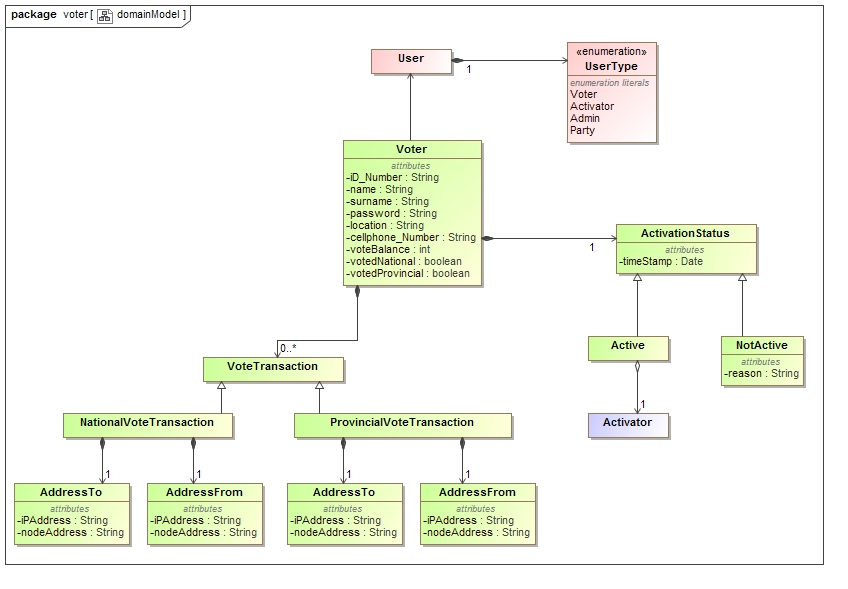
\includegraphics[width=0.75\linewidth]{../Images/DomainModels/voter_domainModel.png}
				\caption{Voter Domain Model}
			\end{figure}
			
			*insert discription here*
			\newline
			\item \textbf{Party}
			\begin{figure}[H]
				\centering
				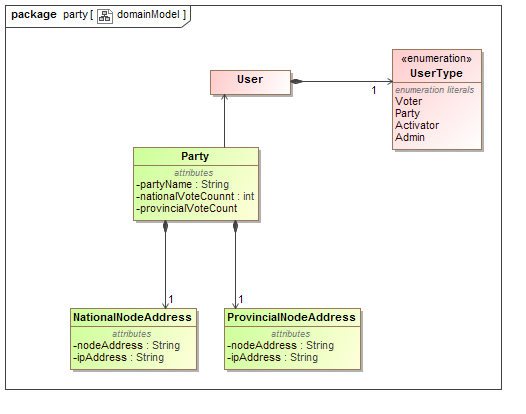
\includegraphics[width=0.75\linewidth]{../Images/DomainModels/party_domainModel.png}
				\caption{Party Domain Model}
			\end{figure}
			
			*insert discription here*
			\newline
			\item \textbf{Admin}
			\begin{figure}[H]
				\centering
				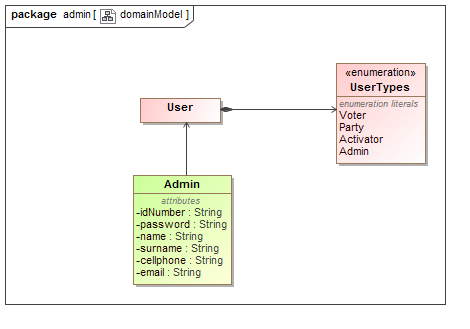
\includegraphics[width=0.75\linewidth]{../Images/DomainModels/admin_domainModel.png}
				\caption{Admin Domain Model}
			\end{figure}
			
			*insert discription here*
			\newline
			\item \textbf{Activator}
			\begin{figure}[H]
				\centering
				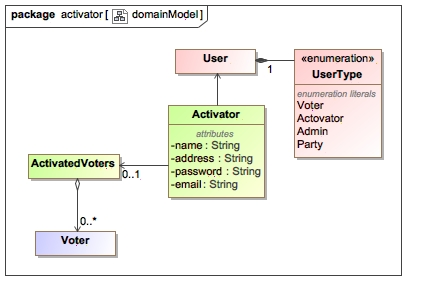
\includegraphics[width=0.75\linewidth]{../Images/DomainModels/activator_domainModel.png}
				\caption{Activator Domain Model}
			\end{figure}
			
			*insert discription here*
			\newline
\end{enumerate}
		
	\section{Open Issues}
		\subsection {GitHub Repository}
	\begin{enumerate}
		\item[] For more information and/or further references, please follow this \href{https://github.com/ish1993/eVoting}{link}, for access to Team CodeX's github repository.
	\end{enumerate}
	
\end{document}